\subsection{GraphBLAST GraphBLAS}

%% ToDo: Carl

GraphBLAST~\cite{Yang:2019:GBL} is the first high-performance GPU (graphics processing unit) implementation of GraphBLAS. Inspired by the design of GBTL, the architecture of GraphBLAST is also C++ based and maintains a separation of concerns between a top-level interface defined by the GraphBLAS C API specification and the low-level backend. One novel aspect about GraphBLAST is that it supports performance-oriented optimizations such as  direction-optimization (also known as push-pull traversal), which was discovered by Beamer, Asanovic and Patterson~\cite{Beamer:2012:DOB} and generalized by Shun~\cite{Shun:2013:Ligra} to other graph algorithms.

Yang, Bulu\c{c} and Owens~\cite{Yang:2018:IPE} show that this optimization is key for a GraphBLAS implementation to meet the performance of state-of-the-art graph frameworks on the GPU like Gunrock~\cite{Wang:2017:GGG}. In each iteration of an \verb'GrB\_mxv', the GraphBLAST backend checks whether the vector sparsity was has crossed a threshold $k$. If it has gone above the threshold, then the traversal will switch from push to pull. If it has gone below the threshold, then the traversal will switch from pull to push. If neither outcome has occurred, then it will use the traversal it used in a previous iteration. 

To support direction-optimization, the GraphBLAST backend maintains a SparseVector and DenseVector object as shown in Figure~\ref{fig:graphblast}. An environmental variable.The push traversal is performed using Gustavson's method as a sparse-matrix sparse-vector multiply (SpMSpV) between the SparseVector and the adjacency matrix transpose in CSC format. The pull traversal is performed in a dot-product manner as a sparse-matrix dense-vector multiply (SpMV) between the DenseVector and the adjacency matrix in CSR format. This raises the issue of having to keep around two copies of each Matrix object when the Matrix is not symmetric. An environmental variable is used to control whether the user want this performance-oriented storage, or whether they want a more memory-inexpensive storage of only CSR or only CSC in which case the direction-optimization feature is disabled.

\begin{figure}[t]
	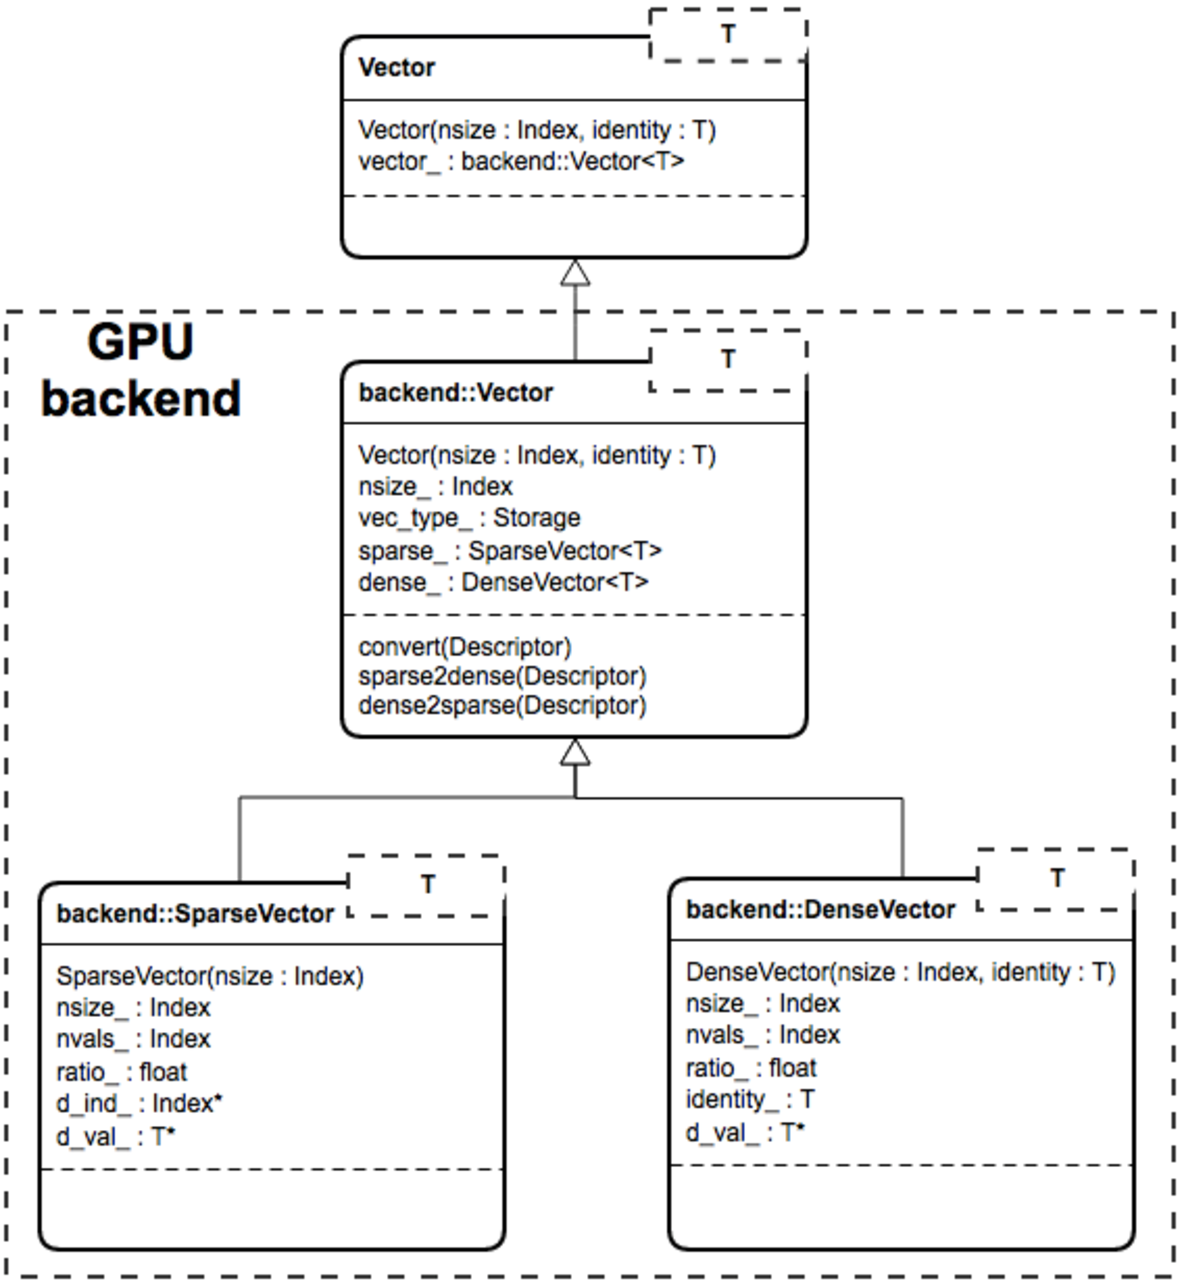
\includegraphics[width=\linewidth]{fig/graphblast}
	\label{fig:graphblast}
	\caption
	{\textbf{GraphBLAST Vector UML diagram.}}
\end{figure}